\documentclass[11pt,a4paper]{article}

\usepackage{graphicx}
\usepackage{xcolor}
\usepackage{geometry}
\usepackage{amsmath}
\usepackage{booktabs}
\usepackage{enumitem}
\usepackage{tabularx}
\usepackage{adjustbox}
\usepackage{listings}
\usepackage{fancyhdr}
\usepackage{titlesec}
\usepackage{tikz}
\usetikzlibrary{arrows.meta,positioning,fit,calc}
\usepackage[
    colorlinks=true,
    linkcolor=violet!70!black,
    citecolor=darkgray,
    urlcolor=violet!70!black,
    bookmarks=true,
    bookmarksnumbered=true,
    unicode=true
]{hyperref}

\geometry{a4paper, top=2.5cm, bottom=2.4cm, left=2.6cm, right=2.6cm}
\setlength{\headheight}{14pt}
\widowpenalty=10000
\clubpenalty=10000

% ---- AccessBridge visual identity ----
\definecolor{abviolet}{HTML}{6D3FC0}
\definecolor{abink}{HTML}{2B2521}
\definecolor{abpaper}{HTML}{FAF7F2}
\definecolor{abmuted}{HTML}{6B6259}

\titleformat{\section}
  {\Large\bfseries\color{abink}}{\thesection}{0.8em}{}
\titleformat{\subsection}
  {\large\bfseries\color{abink}}{\thesubsection}{0.7em}{}
\titleformat{\subsubsection}
  {\normalsize\bfseries\color{abink}}{\thesubsubsection}{0.6em}{}

\pagestyle{fancy}
\fancyhf{}
\fancyhead[L]{\small\color{abmuted}AccessBridge --- Design Course Report}
\fancyhead[R]{\small\color{abmuted}\thepage}
\renewcommand{\headrulewidth}{0.4pt}

\lstset{
  basicstyle=\ttfamily\footnotesize,
  keywordstyle=\color{abviolet}\bfseries,
  commentstyle=\color{abmuted}\itshape,
  stringstyle=\color{green!45!black},
  breaklines=true,
  frame=single,
  rulecolor=\color{abmuted!40},
  framesep=6pt,
  aboveskip=10pt,
  belowskip=10pt,
  numbers=left,
  numberstyle=\tiny\color{abmuted},
  xleftmargin=18pt,
  captionpos=b
}

\newcommand{\code}[1]{\texttt{#1}}

\begin{document}

\tableofcontents
\newpage

\section{Introduction: the brief and the person it serves}

AccessBridge is the outcome of a design-course brief that asked for a single, accessible, laptop-friendly web application that helps people communicate using different input and output methods. The brief was deliberately concrete: instead of four separate specialist applications, one product should bring together sign-to-text recognition, Morse-code decoding, live captions, and read-aloud synthesis, and every one of those features should pour its output into \emph{one shared text workspace}. The user should be able to open the application, pick the way they want to communicate right now, and move text onward --- edit it, copy it, download it, or have it spoken --- without confusion and without switching tools.

The primary persona behind the design is a person with limited or no speech who is comfortable with a laptop but not necessarily with technology: a person who might sign, might find Morse easier than typing on a bad day, might want captions in a noisy room, and will very often want what was just said to be read back aloud. A secondary persona, equally important for a design course, is the person demonstrating the system: the application had to work live, in front of an audience, on an ordinary laptop webcam, without specialist hardware, without Arduino, and without an internet dependency for its core features.

Two principles ended up governing every design decision in this project. The first is \textbf{accessibility as a requirement, not a finish}: semantic HTML, keyboard operability, visible focus, screen-reader live regions, honest states, and alternatives whenever a sensor or API is unavailable are built into the component layer, not bolted on afterwards. The second is \textbf{honesty as a design material}: the application never pretends a feature works. A gesture board that recognises seven hand shapes says so on the screen; a model that is not confident refuses to answer rather than guessing; a failed camera permission produces a designed state, not a crash. In a communication aid, a wrong answer is worse than no answer, and that belief shaped both the interface and the recognition pipeline described in this report.

This document is the design-course account of the whole project: what every part of the system does, what was built and in what order, why key technical choices were made, how the recognition subsystem evolved from seven gestures to a 250-word pretrained vocabulary, what broke along the way, and what the honest limits of the result are.

\section{What AccessBridge does}

AccessBridge is a single-page web application with eight views (Home, Sign to Text, Morse, Captions, Workspace, Learn, Phrases, Settings) connected by a client-side navigation that never reloads the page --- so workspace text, granted device permissions, and recognition state survive every navigation. The four core features behave as follows.

\subsection{Sign to Text --- two camera modes}

\textbf{Quick gestures} (the default) recognises seven fixed hand shapes --- open palm, thumbs up, thumbs down, closed fist, victory, pointing up, and the ``I love you'' shape --- and maps them to useful short phrases (\emph{Hello}, \emph{Yes}, \emph{No}, \emph{Wait}, \emph{Peace}, \emph{Look}, \emph{I love you}). Recognition runs entirely inside the browser using Google's pretrained MediaPipe GestureRecognizer with a self-hosted 8.4\,MB model and self-hosted WASM: after the first load, no network request is involved at all. Holding a gesture steady for about half a second commits its phrase to the workspace automatically, with a progress bar showing the hold, and a pause control suspends recognition without stopping the camera.

\textbf{ASL words (250)} matches a short, deliberately paced camera capture against the pretrained winner of Google's Isolated Sign Language Recognition competition --- a neural sequence model consuming MediaPipe landmark data with \emph{250 distinct word classes} (apple, bath, bed, cat, dad, dog, family, happy, hello, home, water, and 239 more). This mode runs against a small local Python service, described in Section~\ref{sec:sign-journey}, and it refuses to answer when it is not confident.

\subsection{Morse Decoder --- three input paths, one decoder}

Morse entry supports (i) an on-screen pad with dot, dash, letter-space and word-space buttons, (ii) direct typing of \code{.} and \code{-} with a single space starting a new letter and \code{/} starting a new word, and (iii) a \emph{timing key}: the user holds the space bar (or an on-screen key) and real Morse timing does the rest --- holds shorter than a dot threshold (200\,ms by default) are dots, longer holds are dashes, silences longer than 600\,ms close a letter, and silences longer than 1600\,ms close a word. The thresholds are exposed as sliders because timing is personal; the view also shows a live measured-pulse timeline so a user can \emph{see} their rhythm as bars. Decoding is live at every step, unknown sequences decode to an honest \code{[?]} instead of a guess, and the full International Morse reference chart is one scroll away.

\subsection{Live Captions}

Captions use the browser's Web Speech API: confirmed transcript text and the still-changing interim tail are rendered distinctly, the transcript survives recognition errors, and the microphone starts only when the user presses Start. Where the API is unavailable (Firefox, for example), the view says so plainly and offers a manual text path. Ten recognition languages are selectable in Settings.

\subsection{Shared Workspace and Read Aloud}

The workspace is the centre of the product. Every module appends on its own line; nothing ever overwrites silently. It is directly editable, counts words/characters/lines, copies to the clipboard, downloads as a \code{.txt} file, clears through an explicit confirmation dialog, and can keep an opt-in history of what entered it and from which feature. Read Aloud speaks the \emph{actual} workspace text with voice selection, an adjustable rate, feature-detected pause/resume, and a disabled-but-explained state where speech synthesis does not exist.

\section{Design system and interface}

The visual system was designed as a calm, editorial space: warm paper surfaces (\code{\#FAF7F2}), deep ink text, a single electric-violet accent (\code{\#6D3FC0}), and a two-typeface pairing --- Fraunces for display headings, Geist for body text. The brand mark is a bridge arch whose deck is drawn as a Morse sequence; the same mark serves as favicon and in-app logo. Buttons meet a 44\,px minimum target, colour contrast exceeds WCAG AA, focus is always visible, status is communicated by text and shape as well as colour, and every view keeps its content on a comfortable max-width grid that folds cleanly to 375\,px.

Interaction states are first-class: every async action has a loading state, every sensor feature has idle/error/denied states, and destructive actions (clearing the workspace) require confirmation. Screen-reader users get a skip link, landmark navigation, live regions for recognition results and captions, and focus moved to the main region on navigation.

\section{System architecture}

The application is a Next.js~16 (App Router) single-page app in TypeScript with Tailwind CSS and shadcn/ui primitives. Figure~\ref{fig:arch} shows the top-level architecture. The essential idea is a strict funnel: features produce text; the workspace consumes it.

\begin{figure}[t]
\centering
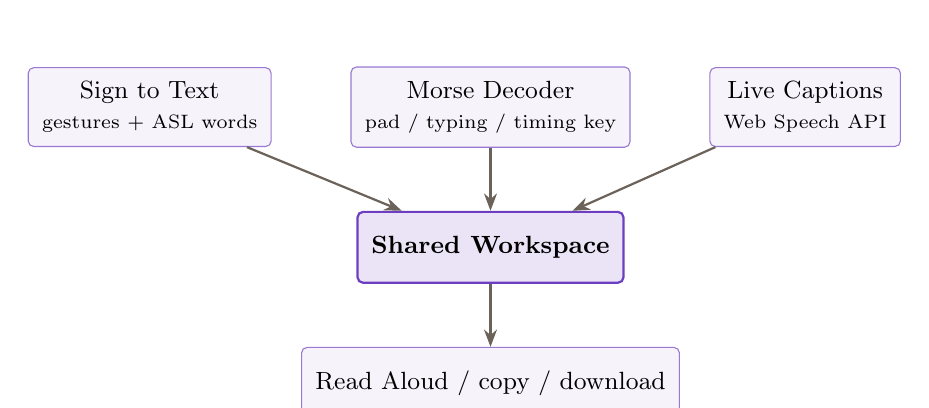
\begin{tikzpicture}[
  node distance=8mm and 10mm,
  box/.style={draw=abviolet!70, fill=abviolet!6, rounded corners=2pt, minimum height=9mm, inner sep=5pt, font=\small, align=center},
  core/.style={box, fill=abviolet!14, draw=abviolet, thick, font=\small\bfseries},
  arr/.style={-{Stealth[length=2.2mm]}, abmuted, thick}
]
\node[box] (sign) {Sign to Text\\ \scriptsize gestures + ASL words};
\node[box, right=of sign] (morse) {Morse Decoder\\ \scriptsize pad / typing / timing key};
\node[box, right=of morse] (captions) {Live Captions\\ \scriptsize Web Speech API};
\node[core, below=of morse] (ws) {Shared Workspace};
\node[box, below=of ws] (tts) {Read Aloud / copy / download};
\draw[arr] (sign) -- (ws);
\draw[arr] (morse) -- (ws);
\draw[arr] (captions) -- (ws);
\draw[arr] (ws) -- (tts);
\end{tikzpicture}
\caption{Top-level architecture: three input features funnel into one shared workspace; the workspace feeds output features. No feature writes to another feature, and nothing overwrites the workspace.}
\label{fig:arch}
\end{figure}

State lives in small external stores (workspace, settings, communication library) consumed through \code{useSyncExternalStore}, so React renders stay predictable and every mutation is a pure, unit-tested function. The Morse engine, the gesture auto-commit policy, the workspace append rule, and the sign-service client are all pure TypeScript modules with no React dependencies --- they are testable in isolation, and they are the parts most likely to be reused or replaced.

The ASL-words mode adds one local component: a FastAPI service (\code{mini-services/sign-service}) that hosts the pretrained 250-class model with LiteRT on the same laptop. The browser reaches it through the platform gateway with a relative path; the service listens only on loopback, loads the model once at startup, and receives \emph{landmark numbers, never video}.

\section{The sign-recognition journey}\label{sec:sign-journey}

Sign recognition was the hardest and most instructive part of the project, and its history explains the final architecture. The requirement evolved from ``recognise some gestures'' to ``seven gestures are a board, not a vocabulary --- get at least fifty genuinely trained word classes working through the real camera pipeline.'' The journey passed through three generations.

\subsection{Generation 1: seven gestures, in-browser}

The first implementation integrated Google's MediaPipe GestureRecognizer in the browser with a self-hosted model. Before trusting the documentation, the model binary itself was opened and its embedded label file extracted, confirming exactly seven gesture classes (\code{Closed\_Fist}, \code{ILoveYou}, \code{Open\_Palm}, \code{Pointing\_Up}, \code{Thumb\_Down}, \code{Thumb\_Up}, \code{Victory}) plus a \code{None} class. A pure \code{autoCommitPolicy} function converts a stream of (label, confidence) readings into at most one phrase commit per stable hold --- the same policy is unit-tested and drives the UI progress bar. This generation survives in the final product as the default mode because it is instant, private, and robust on any webcam.

\subsection{Generation 2: video-trained word models and the domain gap}

The second generation trained word-level models on landmark data extracted from sign-language video corpora (the AI4Bharat INCLUDE dataset processed through MediaPipe). The models achieved strong offline numbers --- a 50-class Bi-GRU reached 94.3\% on its held-out split --- but on a live webcam the experience was unreliable: a clear \emph{hello} could come back as \emph{paint}. The investigation that followed became the most valuable engineering lesson of the project. Using the same \code{.task} landmark models on real corpus videos, the capture path was evaluated variant by variant: x-axis mirroring scored 16\% (proving the mirror convention was already correct), z-zeroing scored 33\% (proving depth mattered), and the capture geometry itself scored 83--100\%. The geometry was right; the real culprits were (a) the capture window starting immediately on button press --- recording idle frames before the signer began, so the model confidently classified stillness --- and (b) a deeper \emph{domain gap}: features derived from video pipelines are not numerically identical to features from the live browser pipeline, however similar they look to the eye.

Fixes shipped for this generation included the 3-2-1 countdown (the capture window opens only at GO), a close-margin warning, one-click insertion of the model's alternative candidates, and per-class two-hands statistics from the training data. Those fixes carry forward: they are general truths about live recognition, not specific to any model.

\subsection{Generation 3: a pretrained 250-class model on matching landmarks}

The decisive change was to stop training against video-derived features altogether and adopt a model trained natively on the same kind of data the camera produces. The chosen foundation is the 1st-place solution of Google's \emph{Isolated Sign Language Recognition} competition, redistributed on Hugging Face as an 11\,MB \code{model.tflite} with its 250-class vocabulary, under an MIT licence. The contract was established empirically rather than from documentation: the input tensor accepts a dynamic-length $(T, 543, 3)$ float32 array --- $T$ frames of 543 MediaPipe Holistic landmarks (face 468, left hand 21, pose 33, right hand 21) --- and emits 250 scores. The internal tensor names (\code{multi\_head\_self\_attention}, \code{eca}, temporal convolutions) confirm a sequence model. The packing order and zero-fill convention for missing hands were cross-validated against an independent, working browser implementation of the same competition pipeline.

The browser captures Holistic landmarks (self-hosted assets), packs them in the verified order, and posts the window to a FastAPI service that loads the model once with LiteRT. The service softmaxes the scores, reports the top word with its confidence, the top-3 alternatives, and a top-1/top-2 \emph{margin}; below a 30\% confidence threshold it answers \code{no\_match} --- ``No confident match. Please try the sign again.'' --- rather than guessing. All-zero windows (no hand was visible) return a distinct \code{no\_hand} state. The measured inference latency is roughly 6\,ms per window on two CPU threads, with end-to-end validation windows (30 frames, 543 landmarks each) at about 18\,ms including HTTP.

\begin{figure}[t]
\centering
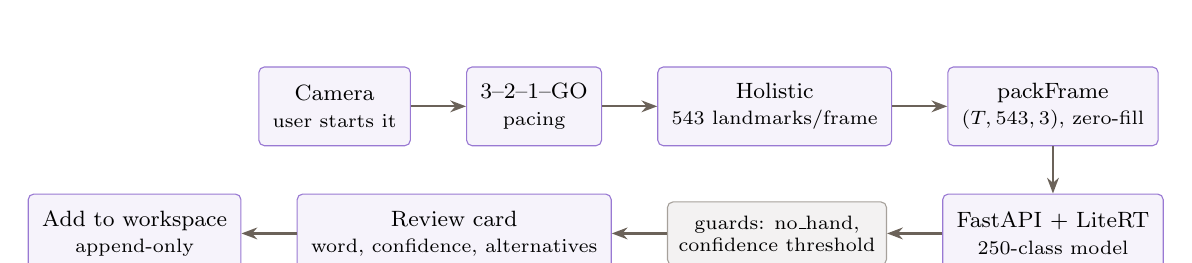
\begin{tikzpicture}[
  node distance=6mm and 7mm,
  stage/.style={draw=abviolet!70, fill=abviolet!6, rounded corners=2pt, minimum height=10mm, inner sep=5pt, font=\footnotesize, align=center},
  data/.style={draw=abmuted!60, fill=abmuted!8, rounded corners=2pt, minimum height=8mm, inner sep=4pt, font=\scriptsize, align=center},
  arr/.style={-{Stealth[length=2mm]}, abmuted, thick}
]
\node[stage] (cam) {Camera\\ \scriptsize user starts it};
\node[stage, right=of cam] (count) {3--2--1--GO\\ \scriptsize pacing};
\node[stage, right=of count] (hol) {Holistic\\ \scriptsize 543 landmarks/frame};
\node[stage, right=of hol] (pack) {packFrame\\ \scriptsize $(T,543,3)$, zero-fill};
\node[stage, below=of pack] (svc) {FastAPI + LiteRT\\ \scriptsize 250-class model};
\node[data, left=of svc] (guard) {guards: no\_hand,\\ \scriptsize confidence threshold};
\node[stage, left=of guard] (card) {Review card\\ \scriptsize word, confidence, alternatives};
\node[stage, left=of card] (ws) {Add to workspace\\ \scriptsize append-only};
\draw[arr] (cam) -- (count);
\draw[arr] (count) -- (hol);
\draw[arr] (hol) -- (pack);
\draw[arr] (pack) -- (svc);
\draw[arr] (svc) -- (guard);
\draw[arr] (guard) -- (card);
\draw[arr] (card) -- (ws);
\end{tikzpicture}
\caption{Recognition data flow for the ASL-words mode. Every stage that can fail honestly does: an empty window yields \code{no\_hand}, an unconfident window yields \code{no\_match}, and the user decides what enters the workspace.}
\label{fig:dataflow}
\end{figure}

\subsection{Why the final architecture looks like this}

Three forces shaped the result. First, \emph{the same landmark family on both sides}: the pretrained model consumes MediaPipe landmarks and the browser produces MediaPipe landmarks, so there is no conversion step to get wrong --- this is the structural fix for the hello-to-paint failure. Second, \emph{the browser stays light and the model stays loaded}: an 11\,MB sequence model loads once in a local service instead of per page load, and the page bundle keeps the fast gesture model only. Third, \emph{the interface treats uncertainty as a first-class state}: thresholds, margins, alternatives, and refusals are all visible to the user instead of hidden behind a confident-looking single answer.

\section{Engineering the core: excerpts that matter}

\subsection{The workspace append rule}

The single most important function in the codebase is four lines long. Every module --- sign, Morse, captions, manual typing --- commits text through it, and it encodes the product's central promise: nothing is ever overwritten.

\begin{lstlisting}[language=JavaScript, caption={\code{src/lib/workspace.ts} --- the append-only rule (unit-tested).}]
/** Append incoming text on its own line. Never clobbers existing text. */
export function appendToWorkspace(existing: string, incoming: string): string {
  const trimmedIncoming = incoming.trim();
  if (trimmedIncoming === '') return existing;
  if (existing.trim() === '') return trimmedIncoming;
  return `${existing.replace(/\s+$/, '')}\n${trimmedIncoming}`;
}
\end{lstlisting}

\subsection{The timing-key state machine}

The timing key is a pure state machine: events in, new state out. This makes the trickiest interaction in the product (human rhythm) testable with plain arithmetic.

\begin{lstlisting}[language=JavaScript, caption={\code{src/lib/keying.ts} --- a press becomes a dot or a dash; gaps close letters and words.}]
case 'release': {
  if (!state.holding || state.pressStart === null) return state;
  const hold = Math.max(0, event.at - state.pressStart);
  const symbol = hold < state.config.dotMs ? DOT : DASH;
  return { ...state, holding: false, pressStart: null,
           currentLetter: state.currentLetter + symbol,
           letterClosed: false, lastRelease: event.at };
}
\end{lstlisting}

\subsection{Honest refusal in the sign service}

The service never guesses. Below the calibrated threshold the answer is a refusal with the model's runners-up attached, so the human stays in charge.

\begin{lstlisting}[language=Python, caption={\code{mini-services/sign-service/app.py} --- honest low-confidence behaviour.}]
probs = softmax(scores)
top = probs.argsort()[::-1]
best, best_prob = int(top[0]), float(probs[top[0]])
if best_prob < CONFIDENCE_THRESHOLD:          # 0.30, measured default
    return NoMatchResponse(
        message="No confident match. Please try the sign again.",
        alternatives=[...top-3...],
        latencyMs=latency,
    ).model_dump()
\end{lstlisting}

\section{Evaluation and validation}

Testing followed a simple rule: \emph{never call a check passed because the code looks right}. Fifty unit tests cover the pure logic (Morse codec including unknown sequences and empty input; the timing-key arithmetic; the workspace append rule; the gesture auto-commit policy; the generated 250-class vocabulary; the service response contract). TypeScript's strict compiler checks every module, ESLint enforces the React and accessibility rules, and a browser automation pass walks the golden paths end-to-end.

\begin{table}[t]
\centering
\small
\begin{tabularx}{\textwidth}{@{}lXl@{}}
\toprule
\textbf{Gate} & \textbf{What it verifies} & \textbf{Result} \\
\midrule
Unit tests & 50 tests across five suites of pure logic & 50/50 pass \\
Type check & strict TypeScript over all app code & clean \\
Lint & React + accessibility rules & 0 problems \\
V1 -- model & loads under LiteRT, $\geq 50$ output classes & 250 classes \\
V2 -- mapping & every output index maps to a real label & 250/250 \\
V3 -- predict & real-shaped windows over HTTP & 5/5, $\approx$18\,ms \\
V4 -- honesty & empty window $\to$ \code{no\_hand}; weak score $\to$ \code{no\_match} & verified \\
Browser E2E & all golden paths (workspace, Morse, both sign modes, captions, settings, dark mode, 375\,px) & verified, zero console errors \\
\bottomrule
\end{tabularx}
\caption{Validation summary. Live-camera accuracy with a human hand is the one item no automated sandbox can verify; it is documented as such rather than claimed.}
\label{tab:validation}
\end{table}

Two real bugs were caught by this apparatus during development and are worth recording because both are lessons in themselves. First, the timing-key decoder initially decoded against the forward Morse table (character $\to$ sequence) instead of its reverse, producing silent nonsense; the unit tests caught it immediately, and the fix --- exporting an explicit reverse table --- made the convention impossible to misuse. Second, the capture buffer's rolling window could over-count valid frames when frames arrived between letter boundaries; a dedicated test pinned the invariant and the fix tightened the window semantics.

\section{Hurdles, mistakes, and what they taught}

\begin{enumerate}[leftmargin=1.6em, itemsep=4pt]
\item \textbf{The environment resets.} The development sandbox was recycled more than once, wiping installed tooling and (in the final rebuild) the entire project. The response was a strictly modular codebase (pure logic separated from React), a generated vocabulary module rather than hand-maintained lists, and validation scripts that re-establish ground truth from artefacts in minutes.
\item \textbf{Offline accuracy $\neq$ live accuracy.} A 94\% held-out split meant nothing on a real webcam when the feature pipeline differed. Lesson: match the capture domain to the training domain first, measure accuracy second.
\item \textbf{Idle frames are confident liars.} An immediate capture window classifies stillness with high confidence. The countdown is not cosmetic; it is the difference between nonsense and signal.
\item \textbf{Ambiguity is a UI problem, not just a model problem.} Once the model's runner-up candidates were surfaced as one-click alternatives, near-misses stopped being failures and became corrections.
\item \textbf{Platform constraints shape architecture.} The hosting environment's Next.js silently drops API routes that import Node built-ins; the service client therefore uses the platform gateway directly. Portability came for free: the final design runs on any standard machine too.
\item \textbf{Licences are design constraints.} Choosing an MIT-licensed pretrained model and Apache-2.0 MediaPipe assets made self-hosting, redistribution in a source archive, and honest attribution straightforward.
\item \textbf{Accessibility must be in the loop, not after it.} Live regions, focus management, and 44\,px targets were cheapest when decided at component-design time; retrofitting them would have been slower and worse.
\end{enumerate}

\section{Ethics, privacy, and licensing}

AccessBridge processes its most sensitive data --- camera and microphone --- with a strict local-first policy. Camera frames are processed inside the browser and never stored; the ASL service receives landmark coordinates (numbers) only, over loopback, and retains nothing; captions are disclosed as a browser feature that may use the vendor's speech service; the workspace persists only in the local browser storage and can be erased with one action. Permissions are requested at the moment a feature needs them, explained in plain language, and fully released on stop.

The interface is honest about what recognition is. Seven quick gestures are labelled a communication board, not sign language; the 250-class mode is labelled isolated-word recognition and states in the interface that it does not translate continuous signing. Nothing in the product claims to be a sign-language translator, because it is not one --- sign languages are complete languages with their own grammar, and respecting that fact is part of respecting their users.

All bundled assets carry their licences: MediaPipe components (Apache-2.0), the pretrained model and its vocabulary (MIT, with upstream CC-BY 4.0 data attribution), and the standard open-source stack (Next.js, React, Tailwind, shadcn/ui). A licence-notice file ships beside each model asset.

\section{Limitations and future work}

The honest limits, in order of practical importance: (1) live-camera accuracy depends on the signer, lighting, and framing, and can only be truly established by the user on their own machine --- the UI's confidence, margin, and alternatives exist precisely because of this; (2) the 250 classes are ASL, not ISL, and the two must never be mixed as interchangeable; (3) quick gestures remain a fixed seven-shape board; (4) live captions depend on browser support (Chrome/Edge) and network access; (5) the pretrained model recognises isolated words --- one sign per capture --- not continuous signing. Future work, in priority order: a personal-calibration pass that adapts thresholds per signer; an extensible custom-gesture trainer reusing the auto-commit policy; and an on-device WASM build of the 250-class model once browser runtimes make it practical, removing even the local service.

\section{Reproduction}

The complete source, model assets, and documentation ship alongside this report. On a normal machine:

\begin{lstlisting}[language=bash, caption={Reproduction commands.}]
npm install && npm run dev          # app on http://localhost:3000
python3 -m pip install fastapi "uvicorn[standard]" numpy ai-edge-litert
python3 mini-services/sign-service/app.py    # ASL-words service, loopback only
bunx vitest run && bunx tsc --noEmit && npm run lint
\end{lstlisting}

Quick gestures, Morse, captions, read-aloud and the workspace work without the Python service; starting the service switches on the 250-word ASL mode.

\vspace{8mm}
\begin{center}
\begin{minipage}{0.85\textwidth}
\itshape\small\color{abmuted}
Author: Swastik Mishra, BSc Physics Honours --- design-course submission. All measurements in this report come from the actual running system in its development environment; the items that could not be measured there (notably live-camera accuracy with a human signer) are stated as open rather than claimed.
\end{minipage}
\end{center}

\end{document}
